\begin{figure}[h!]
     \centering
    \captionsetup[sub]{font=small}
     \begin{minipage}[h!]{1.1\textwidth}
         \begin{subfigure}[b!]{0.2 \textwidth}
             \caption{$\theta = -\pi$}
             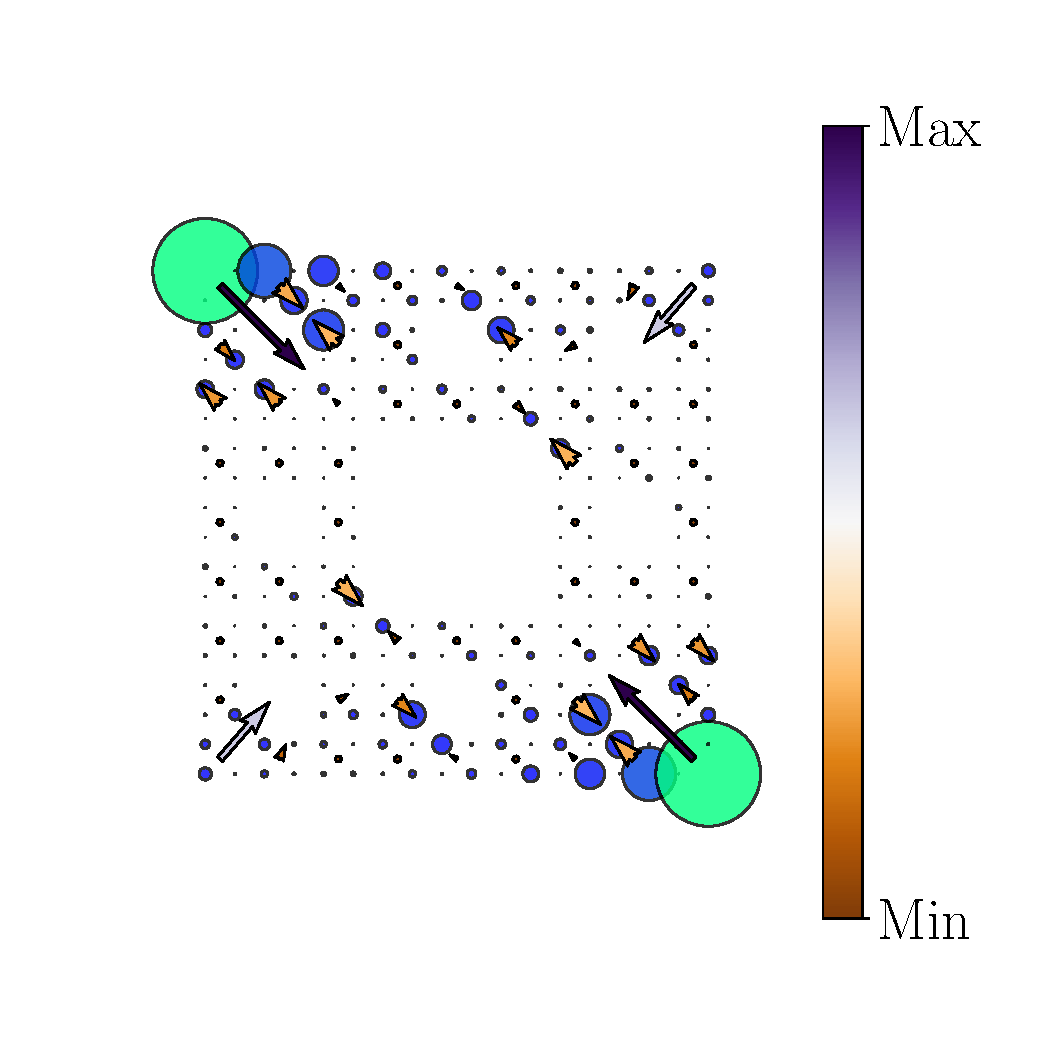
\includegraphics[width=\textwidth]{Imagenes/Resultados_pump_Fractal/y/hoti_pomp_y_pos1.pdf}
         \end{subfigure}\hspace*{-0.5em}
          \begin{subfigure}[b!]{0.2 \textwidth}
             \caption*{$\theta = -\frac{\pi}{2}$}
             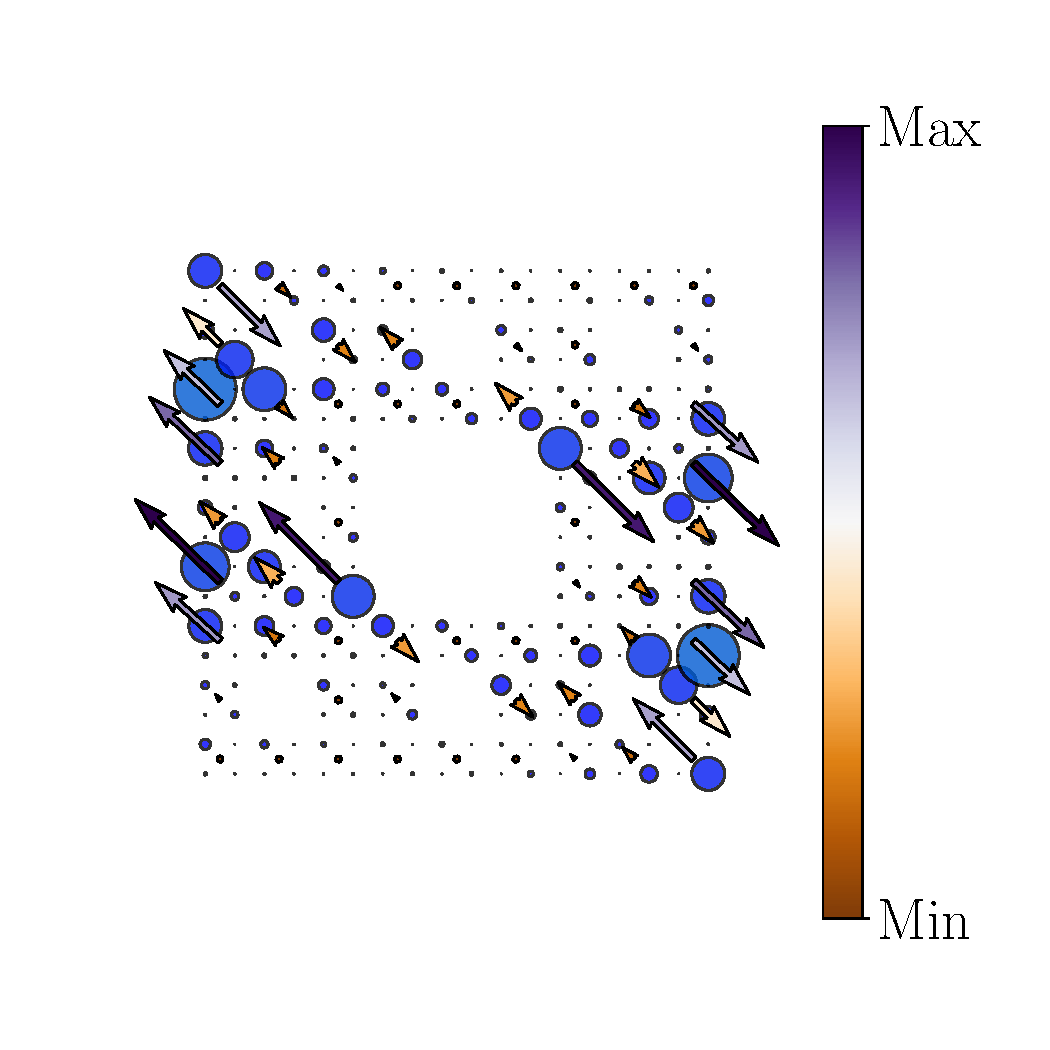
\includegraphics[width=\textwidth]{Imagenes/Resultados_pump_Fractal/y/hoti_pomp_y_pos2.pdf}
         \end{subfigure}\hspace*{-0.5em}
          \begin{subfigure}[b!]{0.2 \textwidth}
             \caption*{$\theta = 0$}
             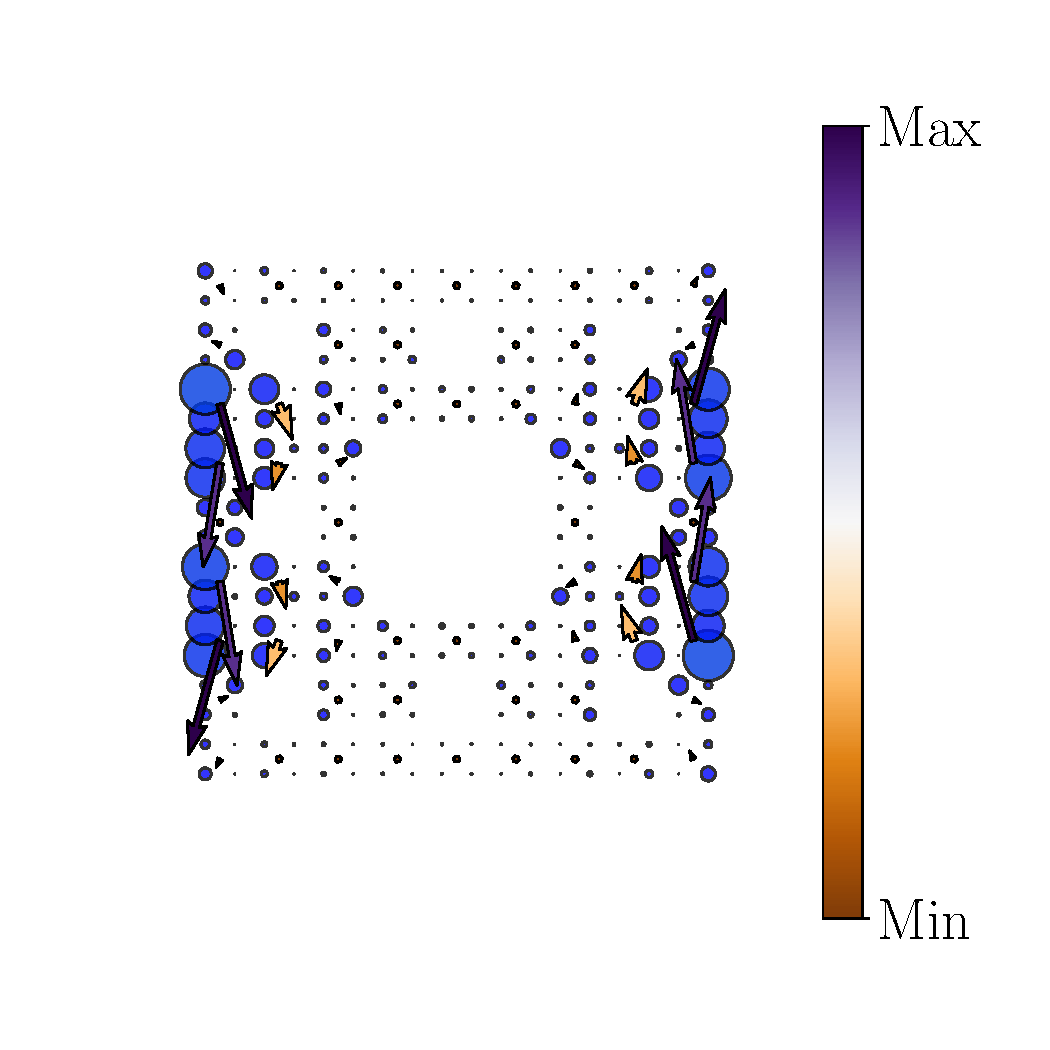
\includegraphics[width=\textwidth]{Imagenes/Resultados_pump_Fractal/y/hoti_pomp_y_pos3.pdf}
         \end{subfigure}\hspace*{-0.5em}
          \begin{subfigure}[b!]{0.2 \textwidth}
             \caption*{$\theta = \frac{\pi}{2}$}
             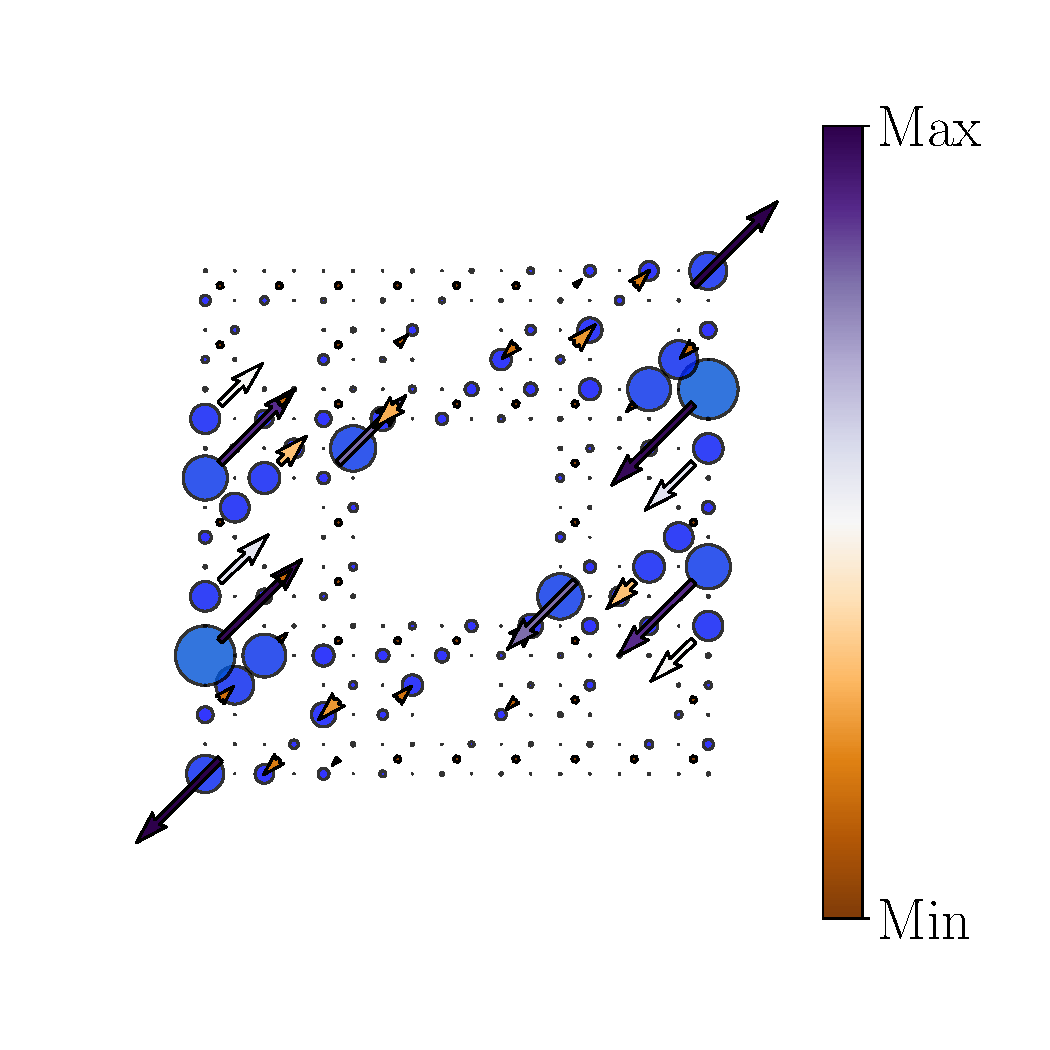
\includegraphics[width=\textwidth]{Imagenes/Resultados_pump_Fractal/y/hoti_pomp_y_pos4.pdf}
         \end{subfigure}\hspace*{-0.5em}
          \begin{subfigure}[b!]{0.2 \textwidth}
             \caption*{$\theta = \pi$}
             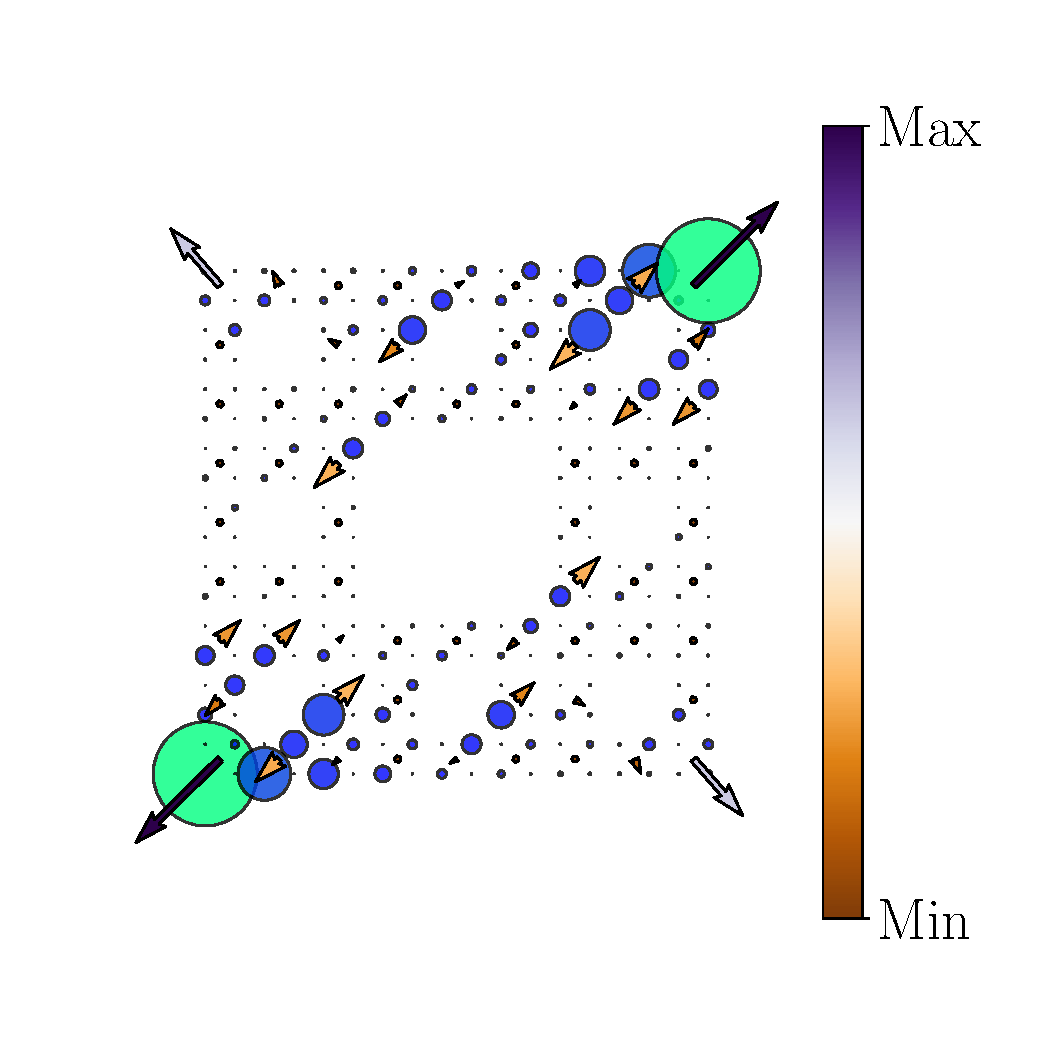
\includegraphics[width=\textwidth]{Imagenes/Resultados_pump_Fractal/y/hoti_pomp_y_pos5.pdf}
         \end{subfigure}\hspace*{-0.5em}
     \end{minipage}\vspace*{-1em}
     
     
     \begin{minipage}[h!]{1.1\textwidth}
          \begin{subfigure}[b!]{0.2 \textwidth}
             \caption{$\theta = -\pi$}
             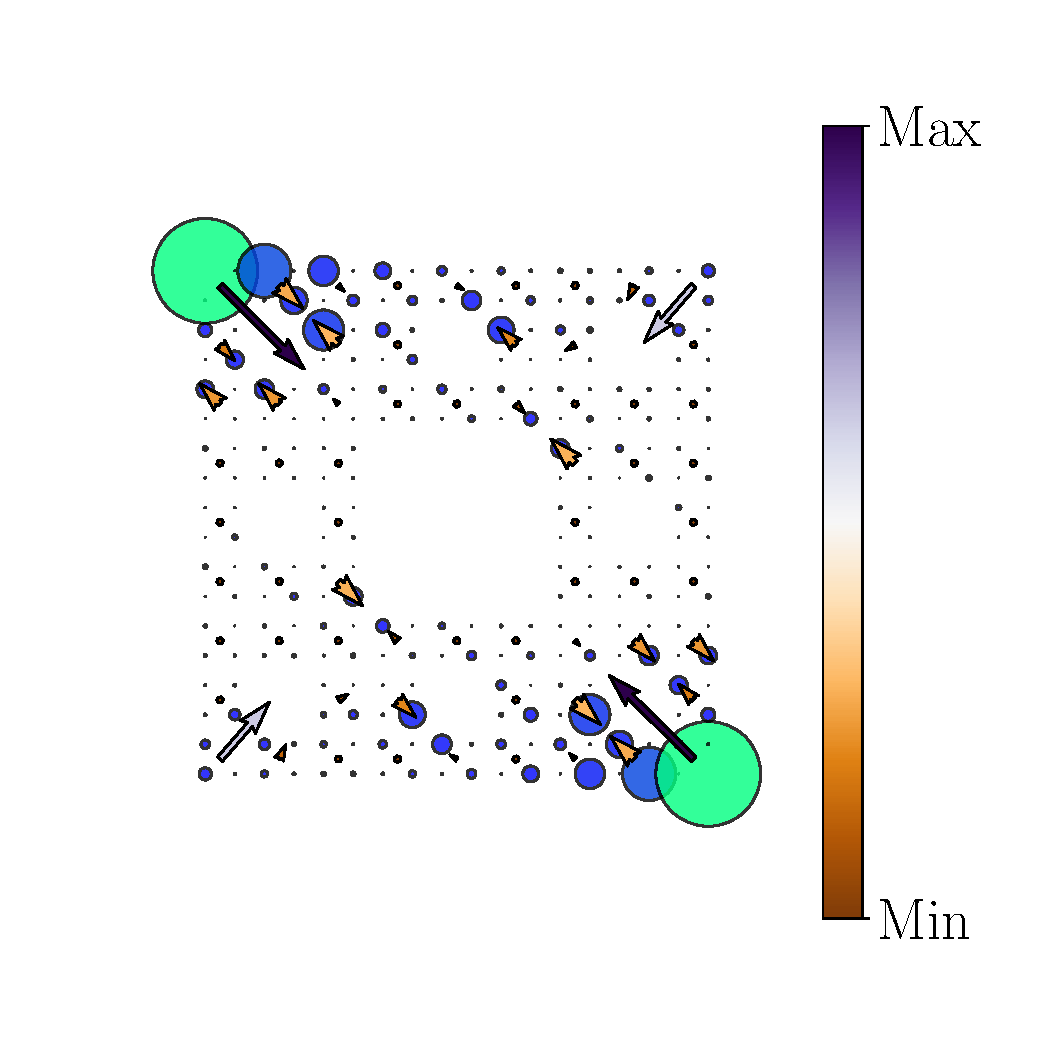
\includegraphics[width=\textwidth]{Imagenes/Resultados_pump_Fractal/y/hoti_pomp_y_neg1.pdf}
         \end{subfigure}\hspace*{-0.5em}
          \begin{subfigure}[b!]{0.2 \textwidth}
             \caption*{$\theta = -\frac{\pi}{2}$}
             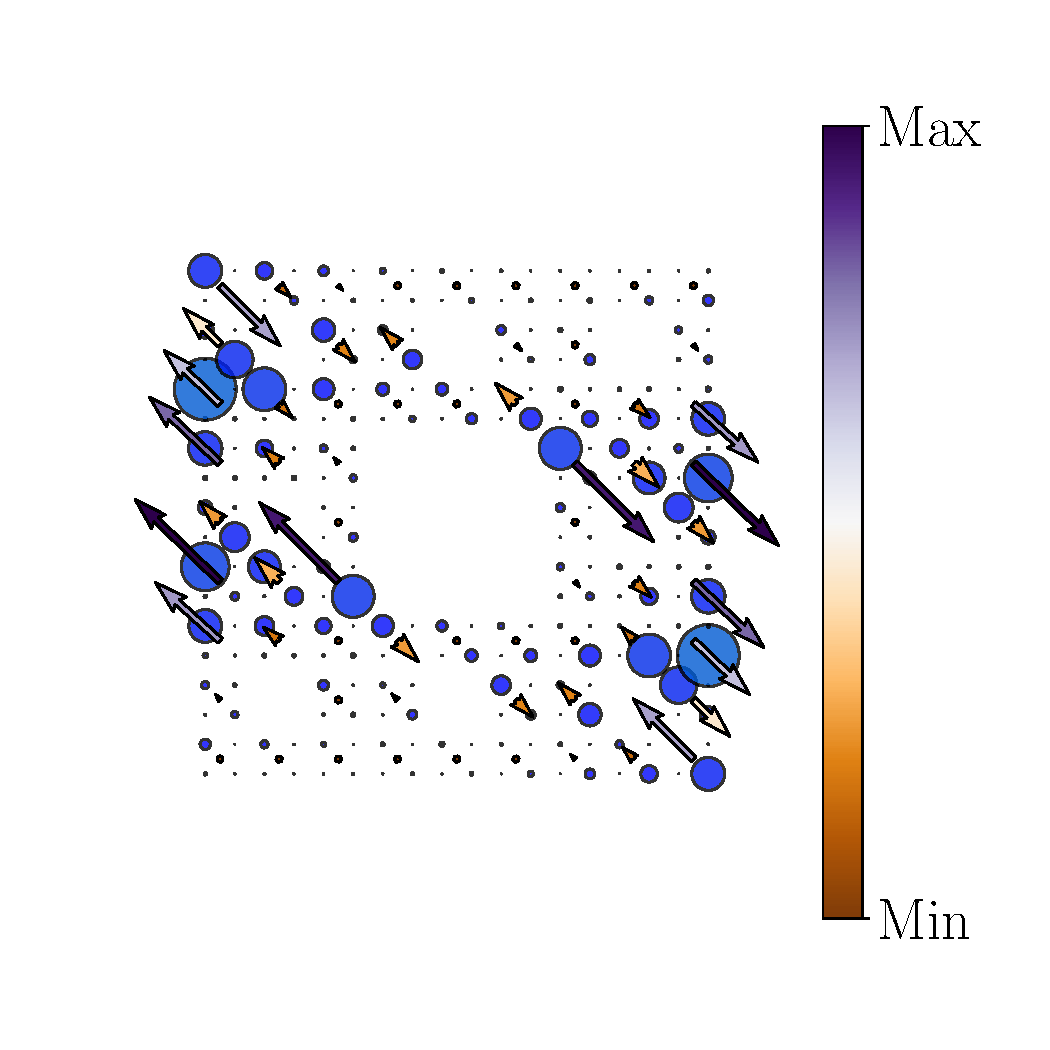
\includegraphics[width=\textwidth]{Imagenes/Resultados_pump_Fractal/y/hoti_pomp_y_neg2.pdf}
         \end{subfigure}\hspace*{-0.5em}
          \begin{subfigure}[b!]{0.2 \textwidth}
             \caption*{$\theta = 0$}
             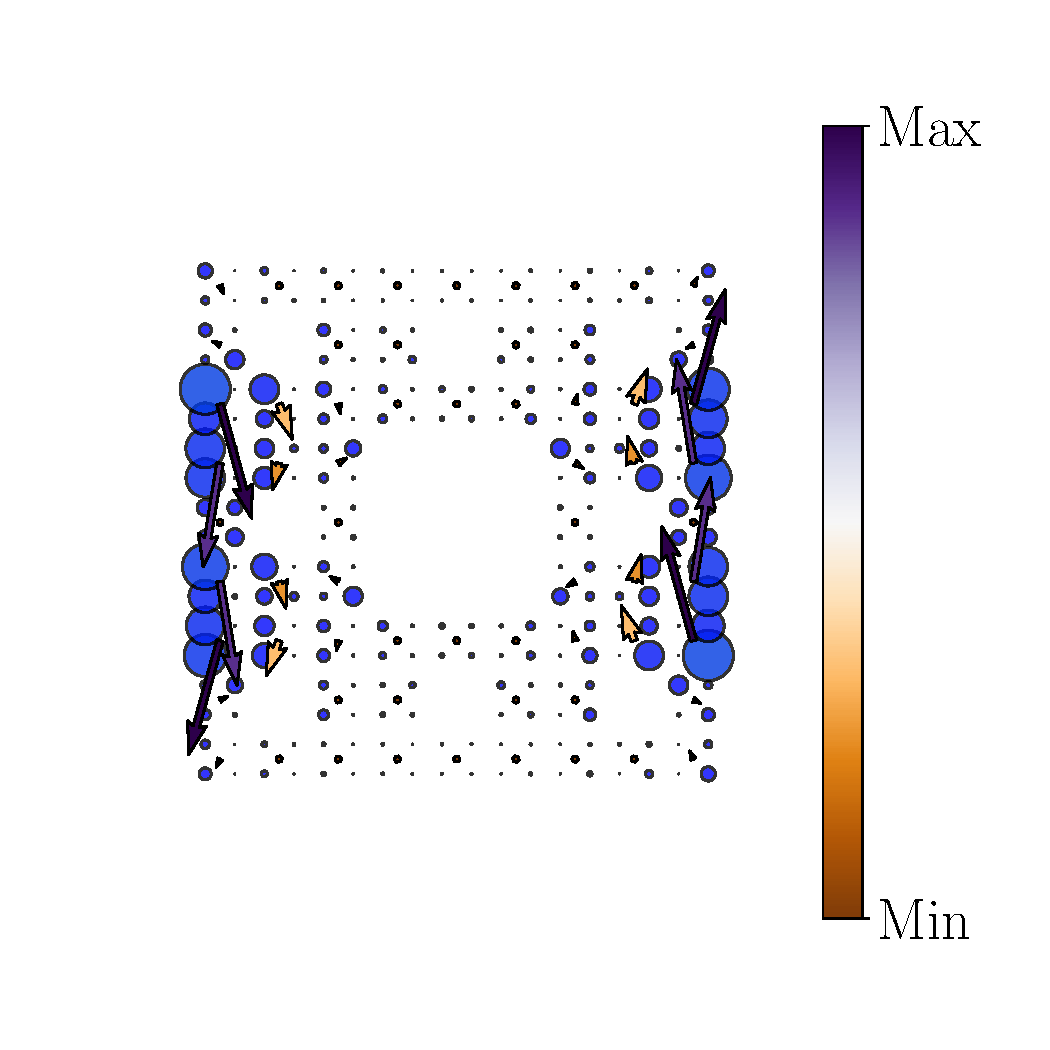
\includegraphics[width=\textwidth]{Imagenes/Resultados_pump_Fractal/y/hoti_pomp_y_neg3.pdf}
         \end{subfigure}\hspace*{-0.5em}
          \begin{subfigure}[b!]{0.2 \textwidth}
             \caption*{$\theta = \frac{\pi}{2}$}
             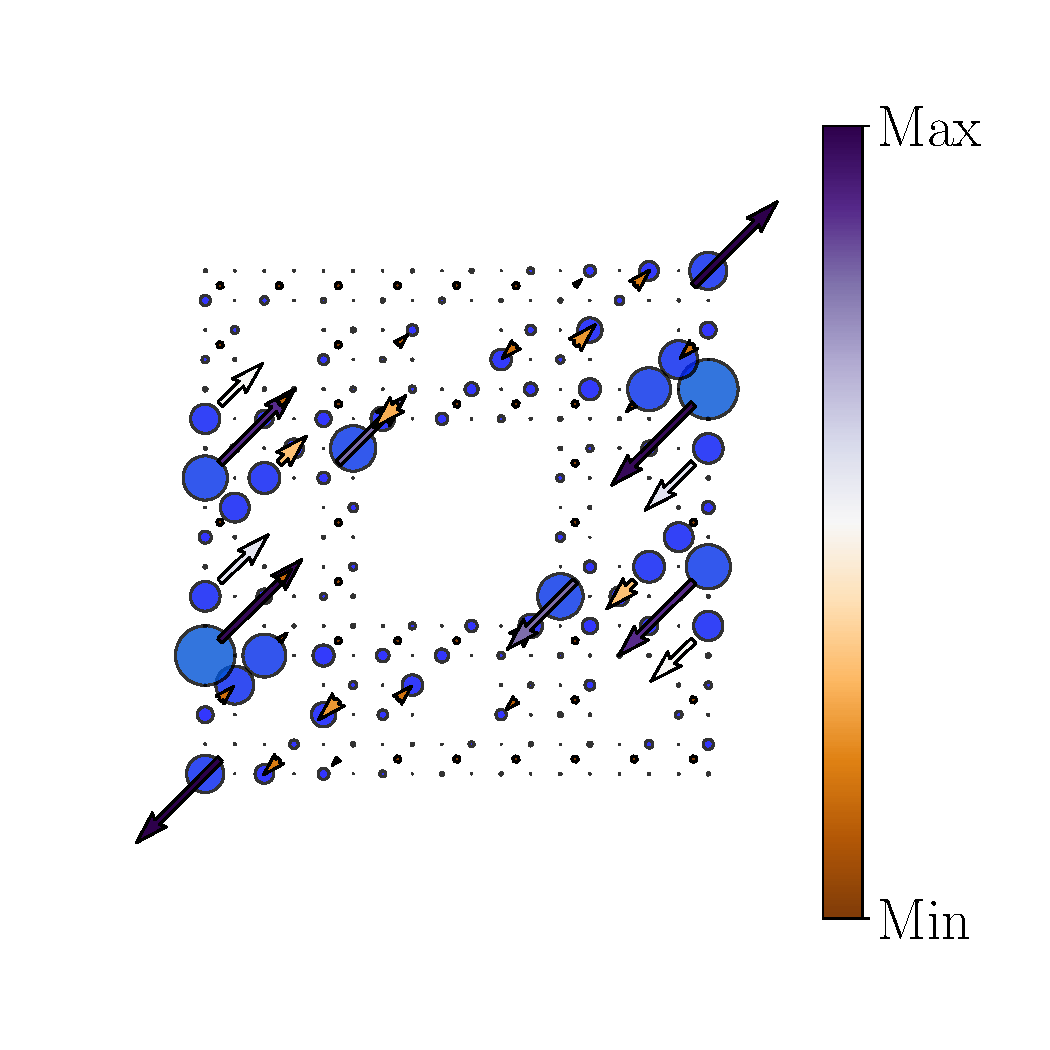
\includegraphics[width=\textwidth]{Imagenes/Resultados_pump_Fractal/y/hoti_pomp_y_neg4.pdf}
         \end{subfigure}\hspace*{-0.5em}
          \begin{subfigure}[b!]{0.2 \textwidth}
             \caption*{$\theta = \pi$}
             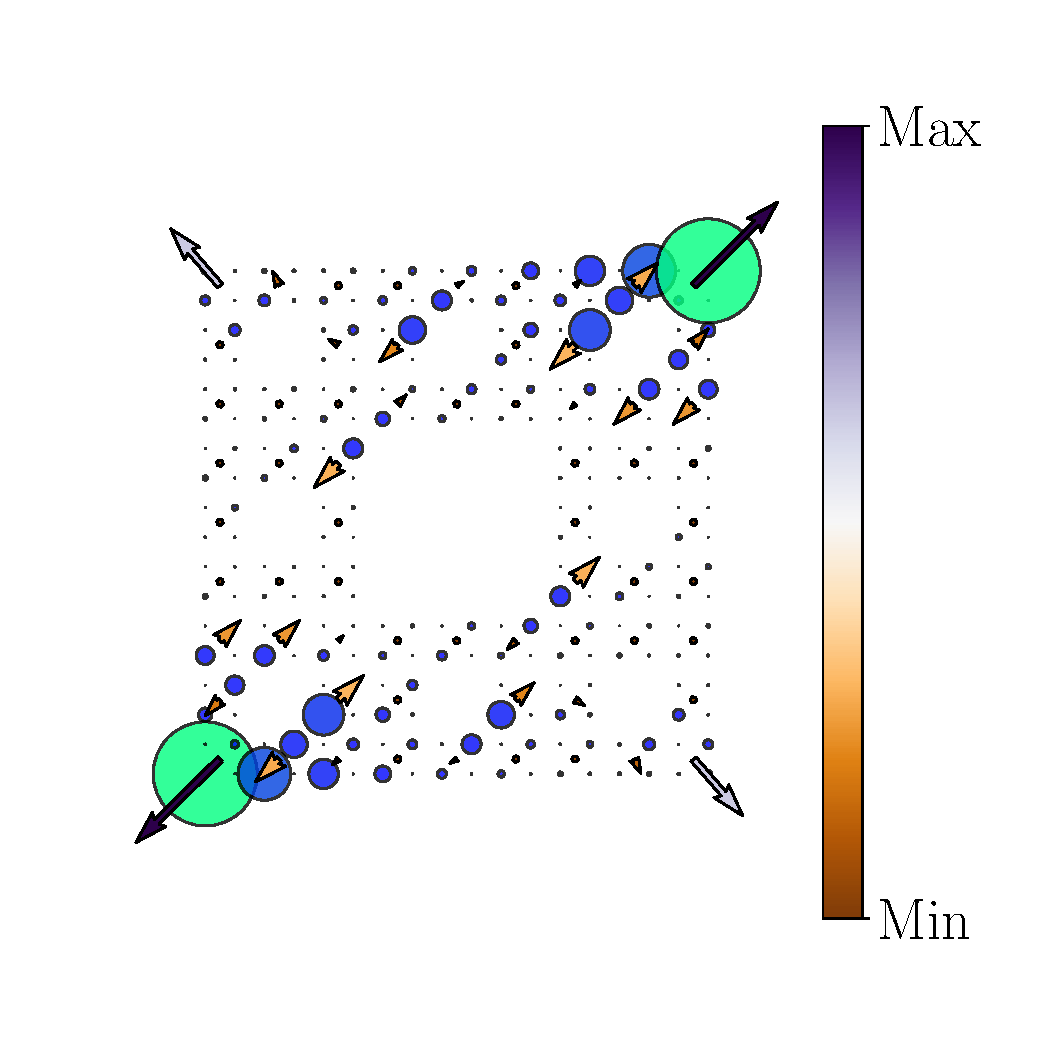
\includegraphics[width=\textwidth]{Imagenes/Resultados_pump_Fractal/y/hoti_pomp_y_neg5.pdf}
         \end{subfigure}\hspace*{-0.5em}
     \end{minipage}\vspace*{-1em}
     
    
     
     
    \caption{\textbf{(a)-(b)} Proyeccion del cambio de la densidad de estados en la red de Sierpinski con bombeo BBH en la dirección \textbf{Y}, las flechas corresponden al flujo de la densidad por celda $\mathbf{J}^{\pm}(\theta)$ [eq. \ref{eq:current_density_cell}]. Las figuras corresponden al especto positivo y negativo de las energias de borde, respectivamente}
    \label{fig:Proy_pump_fractal_y}
\end{figure}